%% ------------------------------------------------------------------------- %%
\chapter{Introduction and Motivation} \label{Chap:Intro}
\lettrine[findent=2pt]{\textbf{T}}{}he parallel and distributed platforms available today become more and more \textit{heterogeneous}.
Such heterogeneous architectures, composed of several kinds of computing units, have had a growing impact on performance in high-performance computing.
Hardware accelerators, such as General Purpose Graphical Processing Units (in short GPUs), are often used in conjunction with multiple computing units (CPUs) on the same chip sharing the same common memory.
As an instance of this, the number of platforms of the ~\cite{TOP500} equipped with accelerators has significantly increased during the last years. In the future it is expected that the nodes of such platforms will be even more diverse than today: they will be composed of fast computing nodes, hybrid computing nodes mixing general purpose units with accelerators, I/O nodes, nodes specialized in data analytics, etc. In order to use all the computational power available, applications should be composed of multiple tasks that allow the usage of the available resources as efficiently as possible. 

The Job Management System (JMS) is the middleware responsible for distributing computing power to applications. A JMS must allocate resources to tasks in order to optimize the use of the available resources while guaranteeing good performance for all applications running in parallel. A promising way to achieve this is using performance prediction. However, in a scenario with millions of processors and a large number of tasks it is very difficult to predict the performance of applications.

Job management systems require that users provide an upper bound of the execution times of their jobs (wall time). Usually, if the execution goes beyond this upper bound, the job is killed. According to~\cite{Gaj:Trystram:2002}, this leads to very bad estimations, with an obvious bias that tends to overestimate this duration. Moreover, those jobs are subject to uncertainties that depend on the context and other running jobs. The uncertain information is generated by communications and executions that depends on the specific context.

The GPUs were initially conceived with the purpose to accelerate the 2D and 3D graphics tasks. However, the evolution of the GPU architectures has gone from a single core to a set of dense arrays of highly parallel cores for more general purpose computation. Not surprisingly, the use of this hardware for parallel computing is a very attractive and it is used in several scientific areas. Moreover, nowadays GPUs can be found in a wide number of electronic devices, just to mention a few: desktops, laptops, smartphones, cars and supercomputers~\citep[chap. 10]{verber2014future}. 

GPUs are integrated with multi-core CPUs with the goal to boost more computational processing power. In this way, the regular users have access to a massively parallel environment when acquiring any kind of these devices. Figure \ref{fig:gflops} shows the theoretical performance and bandwidth reached for those devices, this figure shows a comparison between NVIDIA GPUs and current x86 CPUs. The predominant manufacturer of CPUs are Intel and AMD, and of GPUs are NVIDIA and AMD.

\begin{figure}[htpb]
\centering
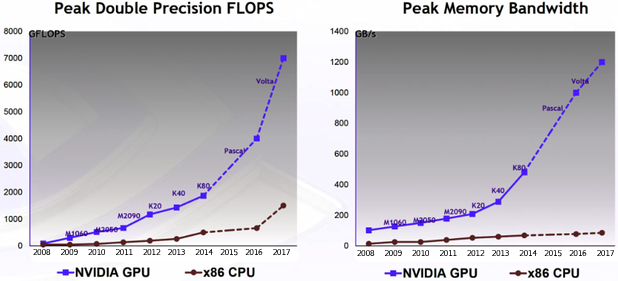
\includegraphics[width=\linewidth]{./images/Volta-GPU.png}
\caption{Theoretical performance and bandwidth reached for recent GPUs. Copied from~\cite{CUDAGuide}}
\label{fig:gflops}
\end{figure}

In GPU applications the computation is done with a large amount of data, which expose restrictions on the storage space available in the devices and the latency of data transfers~\citep{Gregg:2011}. GPUs are composed of hundreds and even thousands of simple cores. Figure~\ref{fig:gpuComp} shows a generic scheme of a heterogeneous system composed of a CPU and a GPU. In this figure we can see that CPUs have much more transistors for control and cache, on other hand GPUs have much more ALUs and few transistors for cache and control. 


\begin{figure}[htpb]
\centering
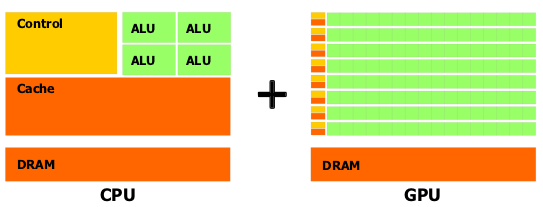
\includegraphics[scale=.85]{./images/gpu-computing.png}
\caption{Multiples Cores CPU + Hundreds or Thousands Cores GPU. Copied from~\cite{CUDAGuide}}
\label{fig:gpuComp}
\end{figure}

Last decade with the development of application programming interfaces for GPUs emerged the concept of General Purpose Computing on GPU or GPGPU. GPGPU has evidenced outstanding results in many scientific areas, however, tools to further capitalize these parallel devices and more refined implementations are still emerging~\citep{CUDAGuide,bsgp}. Researchers in this area can create applications with a concept of parallelism that are able to run on both CPU and GPU architectures. Nevertheless, the implementation of an algorithm, for parallel execution on CPU or GPU, does not guarantee that will execute with the same efficiency in the two architectures. In particular, algorithms with parallelism in large blocks of data, i.e. applications with intensity in array arithmetic and linear data structures, can obtain great benefits when they are implemented for execution exclusively on a GPU~\citep{zhong2012data, Benedict:12}. 

Nowadays, GPUs are general purpose parallel processing units with accessible programming interfaces, including standard languages such as C, Java, and Python. In particular, the Compute Unified Device Architecture (CUDA) is a parallel computing platform that facilitates the development of applications which execute in GPU~\citep{CUDAGuide}. CUDA was introduced by NVIDIA in 2006 for their GPU hardware line. CUDA is a SIMT programming model, it is an extension of SIMD according to Flynn architecture. MIMD is the model used to characterize a machine in an exchange of messages. CUDA is an extension that developers of different languages can use, there is a phase to preprocess the code and extract the CUDA functions. After, CUDA functions are translated into a pseudo-assembly language named PTX  (Parallel Threads eXecution), and the graphics driver contains a compiler which translates the PTX into a binary code which can be run on the processing cores.

CUDA applications are organized in kernels, which are functions executed in GPUs. Kernels are compounded of thread blocks of execution and each one of these blocks can have hundreds or even thousands of threads. Each kernel is executed asynchronously, and various kernels can execute concurrently. The programming model allows directive of synchronization in different levels of the memory hierarchy.

The software development process and performance modeling of GPU applications require a high degree of understanding and knowledge~\citep{Baghsorkhi:2010:APM}. Performance prediction is often just ignored in a development process, this is due to the in-depth analysis that must be done. Models with specific properties to these problems have been created ~\citep{Skillicorn:1998:MLP} to facilitate programming on parallel machines.  Properties such as synchronization and division of work between computing and communication improve the way developers can solve a problem and how the performance of applications running on parallel machines can be modeled.

The accuracy of a GPU performance model is subject to low-level elements such as instruction pipeline usage and cache hierarchy. GPU performance approaches its peak when the instruction pipeline is saturated but becomes unpredictable when the pipeline is under-utilized~\citep{Baghsorkhi:2010:APM}. Effects of cache hierarchy and memory-access divergence are also critical to GPU performance models. Some parallel programs can be efficiently executed on some architectures, but not on others. 

Performance prediction over these devices is a great challenge because hardware characteristics can impact their performance in different ways. There are different approaches to do this, such as analytical modeling and machine learning techniques. Analytic predictive models are useful, but require the manual inclusion of interactions between architecture and software, and may not capture the complex interactions in GPU architectures. Machine learning techniques can learn to capture these interactions without manual intervention but can require large training sets. 

There are different models of parallel machines that help to deal with these problems. Among these models, we have the Parallel Random Access Memory (PRAM), Bulk Synchronous Parallel (BSP) and Coarse Grained Multicomputer (CGM). The main objective of a parallel computing model is to provide a set of parameters that have an impact on the performance of applications in parallel architectures, and thus to be able to simulate the behavior of these applications in their respective architectures.

The Bulk Synchronous Parallel is a computing model for parallel computing introduced for~\cite{Valiant:1990}, BSP model provides a simple but accurate characterization of all parallel machines-past, present, and future. There are other parallel models parameterized, almost all of them using or extending the focus of the BSP model. \cite{Dehne:2002} studied the problem to design scalable parallel geometric algorithms for the Coarse Grained Multicomputer model which are optimal or at least efficient for a wide range of the ratio $\frac{n}{p}$, with $n$ the size of the problem and $p$ the number of processors.

The BSP model allows developers to design algorithms and software that can run on any standard parallel architecture with very high performance~\citep{goldchleger2005implementation}. This model may potentially serve as a unified programming model for both coarse-grained and fine-grained. The model BSP has been implemented as API libraries and programming languages \citep{BSPLib} and API libraries have been developed to use BSP on GPU architectures~\citep{bsgp}, these developments are to create scientific applications in massively parallel environments computing in an easy and better way. Recently, ~\cite{Valiant:2011} has implemented the BSP model over multicore architectures. The implementation of BSP model for multicore architecture incorporates the memory size shared as a further parameter in the computer. The BSP model is a good alternative to tackle parallel problems in massively parallel architectures. 

%Data are produced either by the Job management systems, to effectively leverage these platforms, and by the user's applications that are executed. These applications could be in execution, awaiting execution, monitoring the machine, so forth. While this happens, a lot of information is registered in traces. There are several recent works on using this information~\citep{Tsafrir:Backfilling:2007,Lublin01theworkload,Ernemann:2003}, in other cases these data are ignored by the job management systems~\citep{andreetto2008glite}. 

The developed methods in the area of \textbf{big data} (especially machine learning) can be used for the scheduling of jobs in new computing platforms to large scale. Information about profiling and traces of heterogeneous applications can be used to improve current JMS, which require a better knowledge of the applications~\citep{JMR:Ruiz:2014}. To predict execution or communication times in heterogeneous applications is a great challenge, for this reason, it always is meritorious to research more effective mechanisms to obtain a better performance prediction.

This thesis is related to the modeling and performance prediction of applications executed in GPUs using approaches of analytical model and machine learning techniques. Considering that the market has been taken by NVIDIA graphics cards, our models and experimentation are done on GPUs manufactured by NVIDIA. We evaluated our model using 9 developed kernels and other kernels from Rodinia Benchmark suite~\citep{Rodinia:Che:2009}, Rodinia has been used and accepted by the GPGPU community~\citep{che:2010:Rodinia, nagasaka:2010:Rodinia}, and is used in various GPU simulators~\citep{power:2014:gem5-gpu}.

These CUDA kernels were executed over GPUs with different architectures among these architectures are Kepler, Maxwell, and Pascal. We showed by using profile information for a single board, that the models are general enough to predict the execution time of an application with different input sizes and on different boards.

This thesis also presents the creation of a benchmark, which is freely available in Standard Workload Format (SWF), consisting of five applications of dense linear algebra from the Chameleon software~\citep{agullo2012morse} and a \emph{fork-join} application generated using GGen~\citep{GGen:simutools10}, this benchmark was used for ~\cite{mommessin:2017, mommesin:2017:CCPE} in the experimental evaluation of on-line and off-line scheduling algorithms in machines with heterogeneous resources. 

This benchmark is available online in a web-based hosting service for version control using git, inside the repository, there are a set of application workloads with their respective execution times and dependencies, researchers can use it to test scheduler algorithms of task-based applications over CPU and GPUs. 

%Our model predictions were within $XXXX$ to $XXXX$ times the measured execution times, which are reasonable for such a simple model. These results indicate that the model is good enough to generalize the predictions for different problem sizes and GPU configurations.

\section{Objectives and Thesis Contributions}
The main propose of this work is to present an analysis and design of techniques to predict the performance of applications executed on General-purpose Graphic Processing Units.

In this thesis, we first present an analysis and design of an easy and simple BSP-based model to predict the performance of GPU applications~\citep{amaris:2015:HiPC}. The model is based on the number of computations and memory accesses of the GPU, with additional information on cache usage obtained from profiling. Scalability, divergence, the effect of optimizations and differences of architectures are adjusted by a single parameter.

We also evaluate the use of different machine learning techniques to reach the same objective. We compare three different machine learning approaches: linear regression, support vector machines and random forests with our BSP-based analytical model~\citep{amaris:2016:NCA}. Our main contribution was showing that machine learning techniques provided acceptable predictions for all the applications over all the GPUs. Although the analytical model provided better predictions for some applications, it requires a deep analysis and knowledge of the applications and hardware structure. Consequently, machine learning techniques can be useful for deploying automated on-line performance prediction for scheduling applications on heterogeneous architectures with GPUs, whenever a large data set with information about similar applications is available.

Finally, we developed a benchmark of task-based applications executed on heterogeneous machines. These files are saved in format SWF (Standard Workload Format). This format was defined in order to use a pattern accepted and well used for the community in scheduling research. The benchmark is collected of six parallel applications. Five of them have been created from Chameleon, a dense linear algebra software which is part of the MORSE project~\citep{agullo2012morse}, while the sixth is a fork-join application generated automatically with GGen, a library for generating directed acyclic graphs~\citep{GGen:simutools10}. This benchmark has been tested for \citep{mommessin:2017, mommesin:2017:CCPE}. 

This work was presented in the Doctoral Showcase of the International Conference for High Performance Computing, Networking, Storage and Analysis of 2017. In this conference, a summary of the thesis was presented in a short talk and poster. 

We list the publications directly related to this thesis. %Each one of these papers can be found in the appendix~\ref{app:papers} in the same order as they are presented below.

\begin{itemize}

\bibitem[Amaris {\rm{\em et~al.}} (2015)Amaris, Cordeiro, Goldman, e
  Camargo]{amaris:2015:HiPC}
{\bf Marcos Amaris}, Daniel Cordeiro, Alfredo Goldman e Raphael~Y.de Camargo.
\newblock A simple bsp-based model to predict execution time in gpu
  applications.
\newblock In \emph{High Performance Computing (HiPC), 2015 IEEE 22nd
  International Conference on}, p\'{a}ginas 285--294.
  
\bibitem[Amaris {\rm{\em et~al.}} (2016)Amaris, de~Camargo, Dyab, Goldman, e
  Trystram]{Amaris:2016:NCA}
{\bf Marcos~Amaris}, Raphael~Y.de Camargo, Mohammed~Dyab, Alfredo~Goldman e Denis~Trystram.
\newblock A comparison of GPU execution time prediction using machine learning
  and analytical modeling.
\newblock In \emph{2016 IEEE 15th International Symposium on Network Computing
  and Applications (NCA)}, pages 326--333.

 \bibitem[Mommessin {\rm{\em et~al.}} (2017)Mommessin, Amaris, Lucarelli, e
  Trystram]{Mommessin:2017}
Clement~Mommessin, {\bf Marcos~Amaris}, Giorgio~Lucarelli and Denis~Trystram.
\newblock Generic algorithms for scheduling applications on hybrid multi-core
  machines.
\newblock In \emph{2017 Euro-Par: International Conference on Parallel and
  Distributed Computing}, pages 220--231. 
  
  \bibitem[Mommessin {\rm{\em et~al.}} (2018)Mommessin, Amaris, Lucarelli, e
  Trystram]{mommesin:2017:CCPE}
Clement~Mommessin, {\bf Marcos~Amaris}, Giorgio~Lucarelli and Denis~Trystram.
\newblock Generic algorithms for scheduling applications on heterogeneous multi-core platforms
\newblock \emph{arXiv preprint arXiv:1711.06433} in revision. Submmited in 
\emph{Concurrency and Computation: Practice and Experience}
\end{itemize}  

There are other works which were published during the Doctorate of the candidate and are indirectly related to this thesis:
%\cite{bruel:2015:WSCAD}\cite{gonccalves:2016:HICSS}\cite{okada:2015:WSCAD}\cite{bruel:2017:CCPE}


\begin{itemize}
  \bibitem[Okada {\rm{\em et~al.}} (2015)Okada, Amar{\'\i}s, e vel
  Lejbman]{okada:2015:WSCAD} 
Thiago~Kenji Okada, {\bf Marcos Amar{\'\i}s} e Alfredo~Goldman vel Lejbman.
\newblock Scheduling moldable bsp tasks on clouds.
\newblock In \emph{WSCAD'15 - XVI Simp{\'o}sio em Sistemas Computacionais de
  Alto Desempenho},
    
    \bibitem[Bruel {\rm{\em et~al.}} (2015)Bruel, Amar{\'\i}s, e
  Goldman]{bruel:2015:WSCAD}
Pedro Bruel, {\bf Marcos Amar{\'\i}s} and Alfredo Goldman.
\newblock Autotuning gpu compiler parameters using opentuner.
\newblock In \emph{WSCAD'15 - XVI Simp{\'o}sio em Sistemas Computacionais de
  Alto Desempenho}, pages\'{a}ginas 13--23.
  
  
  \bibitem[Gon{\c{c}}alves {\rm{\em et~al.}} (2016)Gon{\c{c}}alves, Amar{\'\i}s,
  Okada, Bruel, e Goldman]{gonccalves:2016:HICSS}
Rog{\'e}rio Gon{\c{c}}alves, {\bf Marcos Amar{\'\i}s}, Thiago Okada, Pedro Bruel and
  Alfredo Goldman.
\newblock Openmp is not as easy as it appears.
\newblock In \emph{49th Hawaii International Conference on System Sciences}, January-2016,
  pages 5742--5751.

\bibitem[Bruel {\rm{\em et~al.}} (2017)Bruel, Amar{\'\i}s, e
  Goldman]{bruel:2017:CCPE}
Pedro Bruel, {\bf Marcos Amar{\'\i}s} and Alfredo Goldman.
\newblock Autotuning cuda compiler parameters for heterogeneous applications
  using the opentuner framework.
\newblock \emph{Concurrency and Computation: Practice and Experience}
    29\penalty0 (22). 2017
\end{itemize}  

\section{Thesis Outline}
This document is organized into 6 chapters. In Chapter~\ref{chap:characterization}, we show a detailed analysis and characterizations of GPU applications, Chapter~\ref{chap:BSPmodel} shows our proposed BSP-based model used to predict execution times of GPU applications. Chapter~\ref{Chap:ML} presents a machine learning approach for predicting execution times and compare the predictions with those of the analytical model. Chapter~\ref{Chap:Bench} describes the creation of a benchmark of task-based applications executed over heterogeneous resources, CPU and GPUs. Finally we present the conclusions and future works in the Chapter~\ref{chap:conclusion}